\documentclass[hidelinks]{article}
\usepackage[letterpaper,margin=1.0in]{geometry}
\usepackage[utf8]{inputenc}
\pagenumbering{arabic}
\usepackage{authblk}
\usepackage{graphicx}
\usepackage[singlelinecheck=false]{caption} % singlelinecheck makes single line caption left aligned instead of centered
\usepackage{subcaption}
\usepackage{amsmath}
\usepackage[round]{natbib}
\usepackage{fancyhdr}
\usepackage{longtable}
\usepackage{booktabs}
% hyperlinks
\usepackage{hyperref}

\usepackage{xspace}
\usepackage{mathrsfs}
\usepackage{graphicx}

\pagestyle{fancy}
\fancyhead[R]{\textbf{Expanding \stdpopsim}}

% for highlighting text
\usepackage{xcolor}
\usepackage{soul}

% bibliography
\usepackage[round]{natbib}   % omit 'round' option if you prefer square brackets
\bibliographystyle{plainnat}



\newcommand{\Stdpopsim}{\texttt{Stdpopsim}\xspace}
\newcommand{\stdpopsim}{\texttt{stdpopsim}\xspace}

%commands to format figure and table references in the supplement
\newcommand{\beginsupplement}{%
        \fancyhead[L]{Supplemental Material}
        \setcounter{table}{0}
        \renewcommand{\thetable}{S\arabic{table}}%
        \setcounter{figure}{0}
        \renewcommand{\thefigure}{S\arabic{figure}}%
     }
\newcommand{\stopsupplement}{%
        \setcounter{table}{0}
        \renewcommand{\thetable}{\arabic{table}}%
        \setcounter{figure}{0}
        \renewcommand{\thefigure}{\arabic{figure}}%
     }

\makeatletter
\newcommand{\labelname}[1]{\def\@currentlabelname{#1}}
\makeatother

% Avoid pandoc bug when there are lists in the body.
\providecommand{\tightlist}{%
\setlength{\itemsep}{0pt}\setlength{\parskip}{0pt}}

\title{Expanding the \stdpopsim species catalog, and lessons learned for realistic genome simulations}

\author[1]{M. Elise Lauterbur}
\author[2,*]{Maria Izabel A. Cavassim}
\author[3,*]{Ariella L. Gladstein}
\author[4,*]{Graham Gower}
\author[5,*]{Georgia Tsambos}
\author[6,7]{Jeff Adrion}
\author[8]{Arjun Biddanda}
\author[6]{Saurabh Belsare}
\author[6]{Victoria Caudill}
\author[9]{Jean Cury}
\author[10]{Ignacio Echevarria}
\author[11]{Benjamin C. Haller}
\author[12,13]{Ahmed Hasan}
\author[14,15]{Xin Huang}
\author[16]{Leonardo Nicola Martin Iasi}
\author[17]{Jana Obšteter}
\author[18]{Vitor Antonio Corrêa Pavinato}
\author[19,20]{David Peede}
\author[21]{Ekaterina Noskova}
\author[22,23]{Alice Pearson}
\author[24]{Manolo Perez}
\author[6]{Murillo F. Rodrigues}
\author[6]{Chris C. R. Smith}
\author[25]{Jeff Spence}
\author[6]{Anastasia Teterina}
\author[6]{Silas Tittes}
\author[26]{Per Unneberg}
\author[27]{Juan Manuel Vasquez}
\author[28]{Ryan Waples}
\author[29]{Anthony Wilder Wohns}
\author[30]{Yan Wong}
\author[31]{Reed Cartwright}
\author[32]{Aaron P. Ragsdale}
\author[33]{Franz Baumdicker}
\author[34]{Gregor Gorjanc}
\author[35]{Ryan N. Gutenkunst}
\author[30]{Jerome Kelleher}
\author[6]{Andrew D. Kern}
\author[6,36]{Peter L. Ralph}
\author[37]{Daniel R. Schrider}
\author[38]{Ilan Gronau}


\affil[*]{\small{These authors contributed equally to the paper.}}
\affil[1]{\small{Department of Ecology and Evolutionary Biology, University of Arizona, Tucson AZ 85719}}
\affil[2]{\small{Department of Ecology and Evolutionary Biology University of California, Los Angeles}}
\affil[3]{\small{Embark Veterinary, Inc., Boston, MA 02111, USA}}
\affil[4]{\small{Section for Molecular Ecology and Evolution, Globe Institute, University of Copenhagen, Denmark}}
\affil[5]{\small{School of Mathematics and Statistics, University of Melbourne, Australia}}
\affil[6]{\small{Institute of Ecology and Evolution, University of Oregon, Eugene OR 97402}}
\affil[7]{\small{AncestryDNA, San Francisco, CA, 94107, USA}}
\affil[8]{\small{54Gene, Inc., Washington, DC 20005, USA}}
\affil[9]{\small{Université Paris-Saclay, CNRS, INRIA, Laboratoire Interdisciplinaire des Sciences du Numérique, UMR 9015 Orsay, France}}
\affil[10]{\small{School of Life Sciences, University of Glasgow}}
\affil[11]{\small{Department of Computational Biology, Cornell University}}
\affil[12]{\small{Department of Cell and Systems Biology, University of Toronto, Toronto ON}}
\affil[13]{\small{Department of Biology, University of Toronto Mississauga, Mississauga ON}}
\affil[14]{\small{Department of Evolutionary Anthropology, University of Vienna, Djerassiplatz 1, 1030 Vienna, Austria}}
\affil[15]{\small{Human Evolution and Archaeological Sciences (HEAS), University of Vienna, Austria}}
\affil[16]{\small{Department of Evloutionary Genetics, Max Planck Institute for Evolutionary Anthropology, Leipzig, Germany}}
\affil[17]{\small{Agricultural Institute of Slovenia, Department of Animal Science, Hacquetova ulica 17, Ljubljana, Slovenia}}
\affil[18]{\small{Entomology Dept., CFAES, The Ohio State University, Wooster, Ohio}}
\affil[19]{\small{Department of Ecology and Evolutionary Biology, Brown University, Providence, RI, USA}}
\affil[20]{\small{Center for Computational Molecular Biology, Brown University, Providence, RI, USA}}
\affil[21]{\small{Computer Technologies Laboratory, ITMO University, St Petersburg, Russia}}
\affil[22]{\small{Department of Genetics, University of Cambridge, UK}}
\affil[23]{\small{Department of Zoology, University of Cambridge, UK}}
\affil[24]{\small{Department of Genetics and Evolution, Federal University of Sao Carlos, Sao Carlos 13565905, Brazil}}
\affil[25]{\small{Department of Genetics, Stanford University School of Medicine, Stanford, CA, 94305}}
\affil[26]{\small{Department of Cell and Molecular Biology, National Bioinformatics Infrastructure Sweden, Science for Life Laboratory, Uppsala University,  Husargatan 3, SE-752 37 Uppsala, Sweden}}
\affil[27]{\small{Department of Integrative Biology, University of California, Berkeley, Berkeley, CA, USA}}
\affil[28]{\small{Department of Biostatistics, University of Washington}}
\affil[29]{\small{Broad Institute of MIT and Harvard, Cambridge, MA 02142, USA}}
\affil[30]{\small{Big Data Institute, Li Ka Shing Centre for Health Information and Discovery, University of Oxford, OX3 7LF, UK}}
\affil[31]{\small{School of Life Sciences and The Biodesign Institute, Arizona State University, Tempe, AZ USA}}
\affil[32]{\small{Integrative Biology, University of Wisconsin-Madison, Madison, Wisconsin}}
\affil[33]{\small{Cluster of Excellence - Controlling Microbes to Fight Infections, Eberhard Karls Universität Tübingen, Tübingen, Baden-Württemberg, Germany}}
\affil[34]{\small{The Roslin Institute and Royal (Dick) School of Veterinary Studies, University of Edinburgh, Edinburgh EH25 9RG, UK}}
\affil[35]{\small{Department of Molecular and Cellular Biology, University of Arizona, Tucson, Arizona 85721}}
\affil[36]{\small{Department of Mathematics, University of Oregon, Eugene OR 97402}}
\affil[37]{\small{Department of Genetics, University of North Carolina at Chapel Hill, Chapel Hill, North Carolina 27599}}
\affil[38]{\small{Efi Arazi School of Computer Science, Reichman University, Herzliya, Israel}}

\date{\small{\today{}}}

\begin{document}

\maketitle


\section*{Abstract}

Simulation is a key tool in population genetics for both methods development and empirical research,
but producing simulations that recapitulate even the main features of genomic datasets remains a major obstacle.
Today, more realistic simulations are possible thanks to large increases in
the quantity of available data
and the sophistication of inference and simulation software.
However, implementing these simulations still requires substantial time and specialized knowledge.
These challenges are especially pronounced for simulating less well-studied species,
since it is not always clear what level of realism is sufficient
to confidently answer a given question, or what information is required
to produce simulations of that desired realism.
\Stdpopsim is a community-developed framework that seeks to lower this barrier
by making it easy to simulate complex population genetic models using
up-to-date information.
The initial version of \stdpopsim focused on establishing this framework using 
six well-characterized model species.
Here, we report on major updates made in the new release of \stdpopsim (version 0.2),
which includes a significant expansion of the species catalog and substantial additions to simulation capabilities that make it possible to simulate a broader range of species.
Features added to improve the realism of the simulated genomes include non-crossover recombination and provision of species-specific genomic annotations.
Through community-driven efforts, we expanded the number of species in the catalog by more than three-fold and broadened coverage across the tree of life.
Our experience throughout this process was that people are keen to put in the time and effort to include their study species,
but that simple, clear guidance is vital.
Consequently, our intention with this paper is also to provide a learning
modality to meet that need,
by reporting on the main lessons learned through this process
for best practices in population genomic simulation.
We describe the input data required for generating a realistic simulation,
suggest good practices for obtaining the relevant information,
and discuss common pitfalls and major considerations.
These advances to \stdpopsim aim to further promote the use of realistic whole-genome population genetic simulations,
especially in non-model organisms,
making them available, transparent, and accessible to everyone.




\section*{Introduction}
    \label{introduction}

Dramatic reductions in sequencing costs are enabling the generation of
unprecedented amounts of genomic data for a huge variety of species
\citep{Ellegren2014}. Ongoing efforts to systematically sequence life on
Earth by initiatives such as the Earth Biogenome \citep{Lewin2022} and its
affiliated project networks (for example, Vertebrate Genomes
\citep{Rhie2021}, 10,000 Plants \citep{Cheng2018} and others \citep{darwin2022sequence}) are
providing the backbone for enormous increases in the amount of population-level genomic data
available for model and non-model species.
These data are being used to answer questions across scales
from deep evolutionary time to ongoing ecological dynamics.
Methods that use these data, for example to infer demographic history and natural selection,
are also flourishing \citep{Beichman2018}.
While past methods development focused on humans and a few key model systems such as \emph{Drosophila},
more recent efforts are generalizing these methods to include 
important population dynamics not initially accounted for,
such as inbreeding or selfing \citep{Blischak2020}, skewed offspring
distributions \citep{Montano2016}, and intense artificial selection \citep{MacLeod2013, MacLeod2014}.

Simulations can be useful at all stages of this work --
for planning studies, analyzing data, testing inference methods,
and validating findings from empirical and theoretical research.
For instance, simulations provide training data
for inference methods based on machine learning \citep{Schrider2018} and
Approximate Bayesian Computation \citep{Csillery2010}. They can also serve as
baselines for further analyses: for example, simulations incorporating
demographic history serve as null models when detecting selection \citep{Hsieh2016a}
or seed downstream breeding program simulations \citep{Gaynor2020}.
More recently, population genomic simulations have begun
to be used to help guide conservation decisions for threatened species
\citep{Teixeira2021,kyriazis2022using}.

Increasing amounts of data and sophistication of inference methods
have enabled researchers to ask ever more
specific and precise questions. Consequently, simulations must incorporate
more and more detailed elements of a species' biology.
Important elements include genomic features such as mutation and recombination
rates that strongly affect genetic variation and haplotype structure
\citep{Nachman2002}. These have particularly strong ramifications 
when linked selection is important in the patterns of genomic diversity being studied \citep{Cutter2013}.
Furthermore, the demographic history of a species,
encompassing population sizes and distributions, divergences, and gene flow, can
dramatically affect patterns of genomic variation \citep{Teshima2006}. Thus
species-specific estimates of these and other ecological and evolutionary parameters 
(e.g., those governing the process of natural selection) 
are fundamentally important when developing simulations.
This presents challenges, especially to new researchers,
as it takes a great deal of specialized knowledge not only to code the simulations themselves
but also to find and choose appropriate estimates of the parameters underlying the simulation model.

\Stdpopsim is a community resource recently developed to provide easy
access to detailed population genomic simulations \citep{Adrion2020}. It
lowers the technical barriers to performing these simulations
and reduces the possibility of erroneous implementation of simulations
for species with published demographic models. 
The initial release of \stdpopsim was
restricted to only six well-characterized model species, such as
\emph{Drosophila melanogaster} and \emph{Homo sapiens},
but feedback we received from the community identified a widespread desire
to simulate a wider range of non-model species,
and ideally to incorporate these into the \stdpopsim catalog for future use.
This feedback, and subsequent efforts to expand the catalog, 
also uncovered the need for a better understanding of when it is practical to create a realistic
simulation of a species of interest, and indeed what ``realistic'' means in this context.

This paper reports on the updates made in the current release of \stdpopsim  (version 0.2),
and is also intended as a resource for any researcher
who wishes to develop whole-genome simulations for their own species of interest.
We start by describing the main idea behind the standardized simulation framework
of \stdpopsim,
and then outline the main updates made to the \stdpopsim catalog and simulation framework
in the past two years.
We then devote a major section of the paper to provide guidelines for
generating population genomic simulations, either for the purpose of using them in one specific study,
or with the intent of adding these simulations to \stdpopsim.
Among other things, we discuss when a whole-genome simulation is more useful than
simulations based on either individual loci or generic (non-species specific) loci.
We specify the required input data,
mention common pitfalls in choosing appropriate parameters,
and suggested courses of action for species that are missing estimates of some necessary inputs.
We conclude with examples from a couple of species recently added to \stdpopsim,
which demonstrate some of the main considerations involved in the process of designing realistic whole-genome simulations.
While the guidelines provided in this paper are intended for any researcher interested in implementing a population genomic simulation using any software,
we do highlight the ways in which the framework set up by \stdpopsim eases the burden involved in this process.




\section*{The utility of \stdpopsim for genome-wide simulations}
    \label{sec:std-sim}

We begin by providing a brief overview of the importance of genome-wide simulations and the main rationale behind \stdpopsim;
see \citet{Adrion2020} for more on the topic.
The main objective of population genomic simulations is to recreate 
patterns of sequence variation along the genome under known conditions
that model a given species (or population) of interest.
\Stdpopsim is built on top of the
\texttt{msprime} \citep{Kelleher2016,Nelson2020,Baumdicker2022}
and \texttt{SLiM} \citep{Haller2019} simulation engines,
which are capable of producing fairly realistic patterns of sequence variation
if provided with accurate descriptions of the genome architecture
and evolutionary history of the simulated species.
The required parameters include the number of chromosomes and their lengths,
mutation and recombination rates, the demographic history of the simulated population,
and, potentially, the landscape of natural selection along the genome.
A key challenge when setting up a population genomic simulation is to
obtain estimates of all of these quantities from the literature
and then correctly implement them in an appropriate simulation engine.
Detailed estimates of all of these quantities are increasingly available
due to the growing availability of population genomic data
coupled with methodological advances. Incorporating this data
into a population genomic simulation often involves 
integrating this data between different literature sources, which can
require specialized knowledge of population genetics theory.
Thus, the process of coding a realistic simulation can be quite time consuming and often error-prone.

The main objective of \stdpopsim is to streamline this process,
and to make it more robust and more reproducible.
Contributors collect parameter values for their species of interest from the literature,
and then specify these parameters in a template file for the new model.
This model then goes through a vital peer-review process,
which involves recreating the model based on the provided documentation,
and executing automated scripts to compare the two models.
If discrepancies are found in this process, they are resolved by discussion between the contributor and reviewer,
and if necessary with input of additional members of the community.
This quality control process quite often finds subtle bugs \citep[e.g., as in][]{Ragsdale2020}
or highlights parts of the model that are ambiguously defined by the literature sources.
This increases the reliability of the resulting simulations in any downstream analysis.

Another important goal of \stdpopsim is to promote whole-genome simulations,
as opposed to the common practice of simulating many short segments  \citep[see, e.g.,][]{harris2016genetic}.
Simulation of long sequences, on the order of $10^7$ bases,
has until recently been computationally prohibitive,
but this has changed with the development of modern simulation engines,
such as \texttt{msprime} and \texttt{SLiM}.
Generating chromosome-scale simulations has several key benefits.
First, the organization of genes on chromosomes is a key feature of a species' genome that is ignored in many traditional population genomic simulations
 (see \cite{schrider2020background} for a notable exception).
Second, modeling physical linkage allows simulations to capture
important correlations between genetic variants along the same chromosomes.
These correlations reduce variance relative to independent simulations of equivalent genetic material.
This has a particularly striking effect in long stretches of low recombination rates,
as observed for instance on the long arm of human chromosome 22 \citep{Dawson2002}.
In bacteria, a similar effect occurs due to genome-wide linkage that is broken only
by recombination of short segments \citep{Didelot2010}.
When conducting simulations with natural selection, linkage has
an even stronger effect. Selection acting on a small number of sites can
indirectly influence levels and patterns of genetic variation at linked neutral sites,
which has been shown to have a widespread
effect on patterns of genome variation in myriad species
\citep[e.g.,][]{McVicker2009,Charlesworth2012}. 
In addition, the lengths of chromosome-scale shared haplotypes within and
between populations provides valuable information on their demographic history.
Demography inference methods that use such information,
such as MSMC \citep{Schiffels2020}, or IBDNe \citep{browning2015accurate},
perform best on long genomic segments with realistic recombination rates.
Chromosome-scale simulations are clearly required to test (or, train) such methods,
or to conduct power analyses for design of empirical studies that use them.


\section*{Additions to \stdpopsim}
    \label{sec:expanded-catalog}

When first published, the \stdpopsim catalog included six species:
\emph{Homo sapiens}, \emph{Pongo abelii}, \emph{Canis familiaris}, \emph{Drosophila melanogaster},
\emph{Arabidopsis thaliana}, and \emph{Escherichia coli} (Figure \ref{fig:tree}).
One way the catalog has expanded is through introduction of additional demographic models
for \emph{Homo sapiens}, \emph{Pongo abelii}, \emph{Drosophila melanogaster},
and \emph{Arabidopsis thaliana}, enabling a wider variety of simulations for these
thoroughly studied species.
However, the initial collection of six species represents a small slice of the tree of life.
This is a concern
not only because there is a large community of researchers studying other organisms,
but also because methods developed for application to model species (such as humans)
may not perform well when applied to other species with very different biology.
Adding species to the \stdpopsim catalog will allow developers to easily test their methods across a wider variety of organisms.


We thus made a concerted effort
to recruit members of the population and evolutionary genetics community
to add their species of interest to the \stdpopsim catalog.
This effort involved a series of workshops to introduce potential contributors to \stdpopsim, followed by a ``Growing the Zoo'' hackathon organized alongside the 2021 ProbGen conference.
The seven workshops allowed us to reach a broad community of more than 150 researchers,
many of whom expressed interest in adding non-model species to \stdpopsim.
The hackathon was then structured based on feedback from these participants.
One month before the hackathon, we organized a final workshop to prepare interested
participants for the hackathon, by introducing them to  the process of developing
a new species model and adding it to the \stdpopsim code base.
Roughly 20 scientists participated in the hackathon,
which resulted in the addition of 15 species to the \stdpopsim catalog
(Figure \ref{fig:tree}).
The catalog now includes
a teleost fish (\textit{Gasterosteus aculeatus}),
a bird (\textit{Anas platyrhynchos}),
a reptile (\textit{Anolis carolinensis}),
a livestock species (\textit{Bos taurus}),
six insects including two vectors of human disease (\textit{Aedes aegypti} and \textit{Anopheles gambiae}),
a nematode (\textit{Caenorhabditis elegans}),
two flowering plants including a crop (\textit{Helianthus annuus}),
an algae (\textit{Chlamydomonas reinhardtii}),
two bacteria,
four primates and a common mammalian associate of primates (\textit{Canis familiaris}).
Not all of these have genetic maps or demographic models (see Figure \ref{fig:tree}),
but this lays the framework for future contributions.
\begin{figure}
    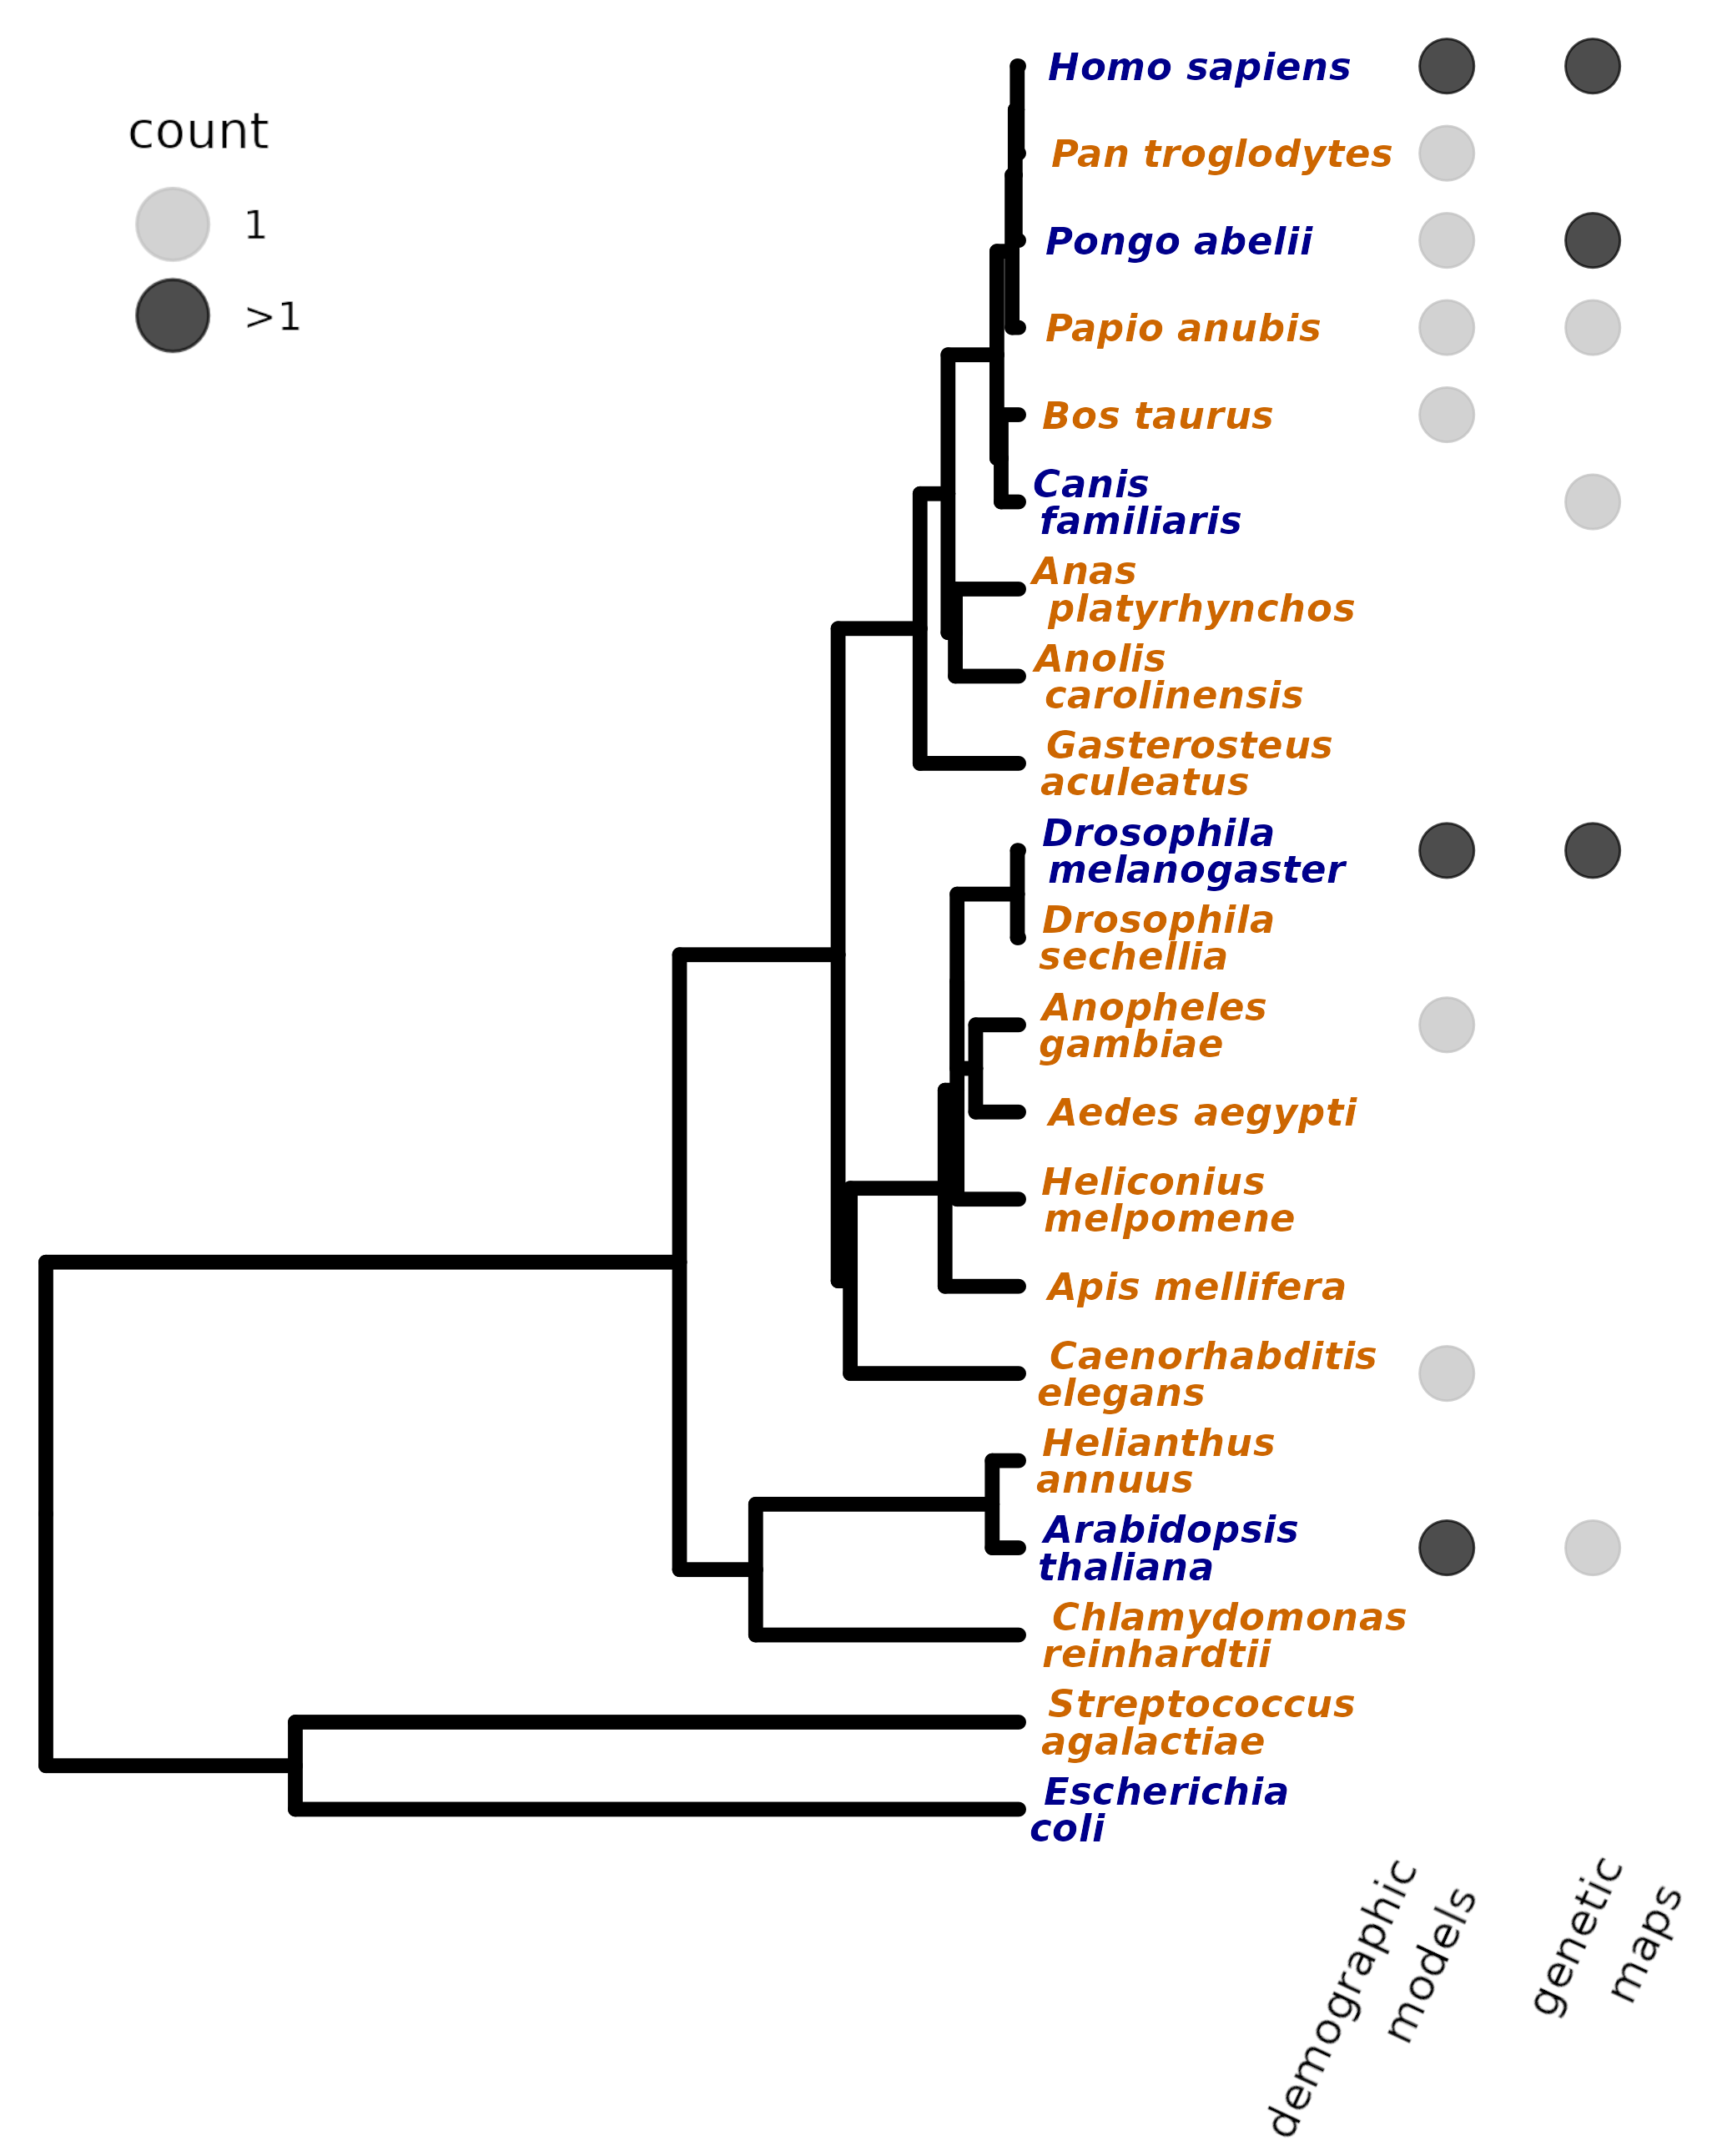
\includegraphics[width=\linewidth]{figs/species_fig}
	\caption{Phylogenetic tree of species available in the \stdpopsim catalog,
		including the six species we published in the original release \citep[in blue]{Adrion2020}, and 15 species that have since been added (in orange).
		Solid circles indicate species that have one (light grey) or more
		(dark grey) demographic models and genetic maps.
		Branch length were derived from the divergence times provided by TimeTree5 \citep{Kumar2022}.
	\label{fig:tree} }
\end{figure}

Expanding the species catalog required adding several functionalities to the simulation framework of \stdpopsim.
Some features were added by upgrading the neutral simulation engine, \texttt{msprime}, from version 0.7.4 to version 1.0. \citep{Baumdicker2022}.
Among other things, this upgrade includes a discrete site model of mutation,
which enables simulating sites with multiple mutations and possibly more than two alleles.
Another key functionality added to the simulation framework of \stdpopsim was modeling of non-crossover recombination.
In bacteria and archaea, recombination occurs primarily through the transfer of DNA segments from one organism to another \citep{Thomas2005,Didelot2010,Gophna2022}.
As a result, such species cannot be realistically simulated with a recombination model that considers only crossovers,
as did the initial version of \stdpopsim.
To address this, we made use of features of the \texttt{msprime} and \texttt{SLiM} simulation engines for modeling non-crossover recombination.
Modeling recombination in a bacterial or (archaeal) species in \stdpopsim is done by setting a flag in the species model to indicate that recombination should be modeled without crossovers,
and specifying an average recombination tract length.
For example, the model for \textit{Escherichia coli} has been updated in the \stdpopsim catalog to use non-crossover recombination at an average rate of $8.9\times 10^{-11}$ (per base per generation),
with an average tract length of 542 bases \citep{Wielgoss2011,Didelot2012}.

Recombination without crossover is also prevalent in sexually reproducing species,
where it is termed \emph{gene conversion}.
Gene conversion affects shorter segments than crossover recombination and creates distinct patterns of genetic diversity along the genome \citep{Korunes2017}.
Indeed, gene conversion rates in some species are estimated to occur at similar or even higher rates than crossover recombination \citep{Gay2007,Comeron2012,Wijnker2013}.
To accommodate this in \stdpopsim simulations,
one needs to specify the fraction of recombinations that occur due to gene conversion (i.e., without crossover), and the average tract length.
For example, the model for \emph{Drosophila melanogaster} has been updated in the \stdpopsim catalog to have a fraction of gene conversions of 0.83 (in all chromosomes with recombination) and an average tract length of 518 bases \citep{Comeron2012}.
We note, however, that since non-crossover recombination incurs a high computation load in simulation,
it is turned off by default in \stdpopsim, and must be explicitly invoked by the simulation model.


Another important extension of \stdpopsim allows augmenting a genome assembly by genome annotations, such as coding regions, promoters, conserved elements, etc.
These annotations can be used to simulate selection at a subset of sites (e.g., the annotated coding regions)
using parametric distribution(s) of fitness effects.
Standardized, easily accessible simulations
that include the reality of pervasive linked selection in a species-specific
manner has long been identified as a goal for evolutionary genetics
\cite[e.g.,][]{McVicker2009,comeron2014background}.
Thus, we expect this extension of \stdpopsim to be transformative in the way simulations are carried out in population genetics.
These significant new capabilities of the \stdpopsim library will be detailed in a forthcoming publication,
and are not the focus of this paper.

\section*{Guidelines for implementing a population genomic simulation}
    \labelname{Guidelines}
    \label{sec:sim-guidelines}


The concentrated effort to add species to the \stdpopsim catalog
has lead to a series of important insights about this process,
which we summarize here as a set of guidelines
for implementing realistic simulations for any species.
Our intention is to provide general guidance that applies to any population genomic simulation software,
but we also mention specific requirements that apply to simulations done in the framework of \stdpopsim.

\subsection*{Basic setup for chromosome-level simulations}

Implementing a realistic population genomic simulation for a species of interest
requires a fairly detailed description of the organism's demography and mechanisms of genetic inheritance.
While simulation software requires unforgivingly precise values,
in practice, we may only have rough guesses for most of  the parameters describing these processes.
In this section, we list these parameters and
provide guidelines for how to set them based on current knowledge.

\begin{enumerate}
\def\labelenumi{\arabic{enumi}.}

\item
  \textbf{A chromosome-level genome assembly}, which consists of a list of chromosomes or scaffolds and their lengths. 
  Having a good quality assembly with complete chromosomes, or at least very long scaffolds, 
  is necessary if chromosome-level population genomic simulations are to reflect the genomic architecture of the species.
  Currently, the number of species with complete chromosome-level assemblies is small,
  but we expect this number to dramatically increase in the near future due to genome initiatives 
  such as the Earth Biogenome \citep{Lewin2022} and its affiliated project networks (e.g.,
  Vertebrate Genomes \citep{Rhie2021}, 10,000 Plants \citep{Cheng2018}).
  Furthermore, the development of new long-read sequencing technologies
  \citep{Amarasinghe2020,Amarasinghe2021} and concomitant advances in assembly pipelines
  \citep{Chakraborty2016} are likely to boost these initiatives. 
  When expanding the \stdpopsim catalog, we decided to focus on species with near-complete 
  chromosome-level genome assemblies (i.e., close to one contig per chromosome).
  This restriction was set mainly because species with less complete genome builds 
  typically do not have good estimates of recombination rate or genetic maps, 
  making chromosome-level simulation much less useful. 
  Therefore, the utility of adding such species to the catalog does not justify the 
  maintenance and storage burden incurred by the large number of contigs in these partial assemblies (see also discussion below).

\item
  \textbf{An average mutation rate} for each chromosome (per generation per bp).
  This rate estimate can be based on sequence data from pedigrees, mutation accumulation studies, 
  or comparative genomic analysis calibrated by fossil data (i.e., phylogenetic estimates).
  At present, \stdpopsim simulates mutations at a constant rate under the Jukes-Cantor model of nucleotide mutations \citep{Jukes1969}.
  However, we anticipate future development will provide support for more complex, heterogeneous mutational processes,
  as these are easily specified in both the \texttt{SLiM} and \texttt{msprime} simulation engines.
  Such progress will further improve the realism of simulated genomes,
  since mutation rates and processes are known to vary along the genome and through time \citep{Benzer1961,Ellegren2003,Supek2019}.

\item
  \textbf{Recombination rates} (per generation per bp).
  Ideally, a population genomic simulation should make use of a chromosome-level \textbf{recombination map}, 
  since the recombination rate is known to vary widely across chromosomes \citep{Nachman2002},
  and this can strongly affect the patterns of linkage disequilibrium and shared haplotype lengths.
  When this information is not available, we suggest specifying an average recombination rate for each chromosome.
  At minimum, an average genome-wide recombination rate needs to be specified, which is typically available for well assembled genomes.
  Recall that for bacteria and archea, which primarily experience non-crossover recombination,
  the average tract length should also be specified
  (see details in previous section).\\
  \textbf{Gene conversion (optional):} If one wishes to model gene conversion in eukaryotes either together with crossover recombination or as a stand-alone process,
  then they should specify the fraction of recombinations done by gene conversion
  as well as the average tract length (per chromosome).

\item
  \textbf{A demographic model} describing 
  ancestral population sizes, split times and migration rates.
  Selection of a reasonable demographic model is often crucial,
  since misspecification of the model can generate unrealistic patterns of genetic variation that will affect downstream analyses \citep[e.g.,][]{Navascues2009}.
  % PLR: an odd citation for that?
  % ILAN: I tried looking for a better one. Will try to crowdsource this
  A given species might have more than one demographic model, fit from different data or by different methods.
  Thus, when selecting a demographic model, one should examine the data sources and methods used to obtain it to ensure that they are relevant to their study.
  At a minimum, simulation requires a single estimate of \textbf{effective population size}. This estimate, which may correspond to some sort of historical average effective population size,
  should reproduce in simulation the average observed genetic diversity in that species. Note, however, that this average effective population size will not capture features of genetic variation that are caused by recent changes in population size and the presence of population structure \citep{MacLeod2013,Eldon2015}.
  For example, a recent population expansion will produce
  an excess of low frequency alleles that no simulation of a constant-sized
  population will reproduce \citep{Tennessen2012}.

\item
  \textbf{An average generation time} for the species.
  This parameter is an important part of the species' natural history.
  This value does not directly affect the simulation, since
  \stdpopsim uses either the Wright-Fisher model (in \texttt{SLiM}) or the Moran model (in \texttt{msprime}),
  both of which operate in time units of generations. 
  Thus, the average generation time is only currently used to convert time units to years, 
  which is useful when comparing among different demographic models.

\end{enumerate}


These five categories of parameters are sufficient for generating simulations
under neutral evolution. Such simulations are useful for a number of purposes,
but they cannot be used to model the influence of natural selection on patterns of genetic variation.
As mentioned above, it is a widely appreciated fact that linked selection modulates
patterns of variation within genomes.
Therefore, its incorporation into simulations is crucial for many purposes.
To achieve this, the simulator needs to know which regions along the genome are subject to selection,
and the nature and strength of this selection.
The current version of \stdpopsim enables simulation with selection
(using the \texttt{SLiM} engine)
by specifying genome annotations and distributions of fitness effects,
as specified below.
We note that the ability to simulate chromosomes with realistic models of
selection is still under development and will be finalized in the next release of \stdpopsim.

\begin{enumerate}
	\def\labelenumi{\arabic{enumi}.}
	\setcounter{enumi}{5}
	\item
	\textbf{Genome annotations}, specifying regions subject to selection (e.g., as GFF3/GTF file).
    For instance, annotations can contain information on the location of coding regions,
    the position of specific genes, or conserved non-coding regions.
    Regions not covered by the annotation file are assumed to be neutrally evolving.

	\item
	\textbf{Distributions of fitness effects} (DFEs) for each annotation.
    Each annotation is associated with a DFE describing
    the probability distribution of selection coefficients (deleterious, neutral, and beneficial)
    for mutations occurring in the region covered by the annotation.
    DFEs can be inferred from population genomic data \citep[reviewed in][]{Eyre-Walker2007},
    and are available for several species \citep[e.g.,][]{Ma2013, Huber2018}.
\end{enumerate}

\subsection*{Extracting parameters from the literature}

Simulations cannot of course precisely match reality, but in setting up simulations
it is desireable to choose parameters that best reflect our current understanding.
In practice a researcher may choose each parameter to match a fairly precise estimate or a wild guess,
which may be obtained from a peer-reviewed publication or from word of mouth.
However, values in \stdpopsim are always chosen to match published estimates,
so that the underlying data and methods are documented and can be validated.
Because the process of converting information reported in the literature to parameters used by a simulation engine is quite error-prone,
some kind of independent validation of the simulation code is crucial.
We highly recommend following a quality control procedure similar to the one used in \stdpopsim,
in which each species or model added to the catalog is independently recreated or thoroughly reviewed by a separate researcher.


Obtaining reliable and citeable estimates for all model parameters is not a trivial task.
Oftentimes, values for different parameters must be gleaned from multiple publications and combined.
For example, it is not uncommon to find an estimate of a mutation rate in one paper,
a recombination map in a separate paper, and a suitable demographic model in a third paper.
Integrating information from different publications requires some care,
because some of these parameter estimates are entangled in non-trivial ways.
For instance, consider simulating a demographic model estimated in a specific paper that assumes
a certain mutation rate.
Naively using the demographic model, as published, with a new estimate of mutation rate
will lead to levels of genetic diversity that do not fit the genomic data.
This is addressed in \stdpopsim by allowing a demographic model to be simulated using a mutation rate that differs from the default rate specified for the species.
See, for example, the model implemented for \emph{Bos taurus},
which is described in the next section.
This important feature does not necessarily fix all potential inconsistencies
caused by assumptions made by the demographic inference method
(such as assumptions on recombination rates).
It is therefore recommended, when possible, to take the demographic model,
mutation rates, and recombination rates from the same study,
and to proceed carefully when mixing sources.
An additional tricky source for inconsistency is coordinate drift between 
subsequent versions of genome assemblies.
In \stdpopsim, we follow the approach from the UCSC Genome Browser
and use liftover to convert the coordinates of genetic maps and genome annotations
that we curate to the coordinates of the genome assembly we use for that species.


\subsection*{Filling out the missing pieces}

\begin{table}[b!]
	\captionof{table}{\textbf{Guidelines for dealing with missing parameters.} %
		For each parameter, we provide a suggested course of action, 
		and mention the main discrepancies between the simulated data
		and real genomic data,
		which can be caused by mis-specification of that parameter.
	} \label{tab:param-mod}
	\begin{tabular}{p{1.5in}p{2.2in}p{2.2in}}
		\hline
		\textbf{Missing parameter}  & 
		\textbf{Suggested action} & 
		\textbf{Possible discrepancies} \\
		\hline
		Mutation rate      &
		Borrow from closest relative with a citeable mutation rate &
		Number of polymorphic sites  \\
		\hline
		Recombination rate &
		Borrow from closest relative with a citeable recombination rate &
		Patterns of linkage disequilibrium
		\\
		\hline
		Gene conversion rate and tract length &
		Set rate to 0 or borrow from closest relative with a citeable rate &
		Lengths of shared haplotypes across individuals
		\\
		\hline
		Demographic model &
		Set the effective population size (Ne) to a value
		that reflects the average observed genetic diversity in the
		simulated population
		     &
		Features of genetic diversity that are captured by the site frequency spectrum,
		such as the prevalence of low-frequency alleles\\
		\hline
	\end{tabular}
\end{table}

For many species it is difficult to obtain estimates of all necessary model parameters.
Table \ref{tab:param-mod} provide suggestions for ways to deal with missing values of various central model parameters.
The table also mentions the main discrepancies between the simulated data and real genomic data,
which can be caused by mis-specification of each parameter.

Several researchers who participated in the ``Growing the Zoo'' hackathon wished to add species
whose genome assemblies are composed of many relatively small contigs,
unanchored to chromosome-level scaffolds.
Although we had not previously put restrictions on which species might be added,
we decided that we would only add species with chromosome-level assemblies.
The main justification for this restriction is that
species with less complete genome builds typically do not have good estimates of recombination rate, genetic maps, and demographic models,
making chromosome-level simulation much less useful in such species.
Another issue is the storage burden and long load times involved in dealing with
hundreds of contigs.
Finally, each species requires validation of its code before it is added to the \stdpopsim catalog,
as well as long-term maintenance to keep it up-to-date with changes made to the \stdpopsim framework.
So, the benefit of including species with very partial genome builds in \stdpopsim
would be outweighed by the substantial extra burden on \stdpopsim maintainers as well as
downstream users of these models.


%Ilan: applied some important edits in this paragraph to better address some of the delicate situations and options we suggest for them 
That being said, simulation is still potentially useful for species with partial genome builds.
Longer contigs or scaffolds in these builds can be simulated separately and independently.
This approach allows us to model genetic linkage within each contig,
but linkage between different contigs that map to the same chromosome will not be captured by the simulation.
This provides a reasonable approximation for many purposes, at least for genomic regions far from the contig edges.
For shorter contigs, separate independent simulations will not be able to capture patterns of long-range linkage in a reasonably realistic way.
Thus, a viable option for shorter contigs is to lump them together into longer pseudo-chromosomes, trying to mimic the species' expected chromosome lengths.
Despite their somewhat artificial construction,
these pseudo-chromosomes have the important benefit of
capturing patterns of linkage similar to those observed in real genomic chromosomes.
%Ilan: tried to give a few concrete examples here
If, for example, the main purpose of the simulation is to examine the distribution of lengths of shared haplotypes between individuals,
or study patterns of background selection,
then it makes sense to simulate such pseudo chromosomes.
Note, however, that specific genetic correlations between different contigs lumped together will potentially be highly inaccurate.
So, if the main purpose of the simulation is to examine local patterns of genetic variation in certain loci of interest, then it might make more sense to simulate the relevant contigs separately (even if they are short), or to randomly sample several mappings of contigs to pseudo-chromosomes.
Ultimately, the recommended mode of simulation for species with partial genome builds depends on the intended use of the simulated genomes.
Finally, we note that for some purposes it may be sufficient to simulate a large number of unlinked sites \citep{Gutenkunst2009,Excoffier2013},
which can be generated without any sort of genome assembly.
However, this approach would not have the many benefits of whole-chromosome simulations,
which we promote in \stdpopsim.


\section*{Examples of added species}
    \labelname{Examples}
    \label{sec:examples}

In this section, we provide examples of two species recently added to the \stdpopsim catalog,
\textit{Anopheles gambiae} and \textit{Bos taurus},
to demonstrate some of the key considerations of the process.

\subsection*{\texorpdfstring{\emph{Anopheles gambiae} (mosquito)}{Anopheles gambiae (mosquito)}}
    \label{AnoGam}
    
\begin{figure}[b!]
	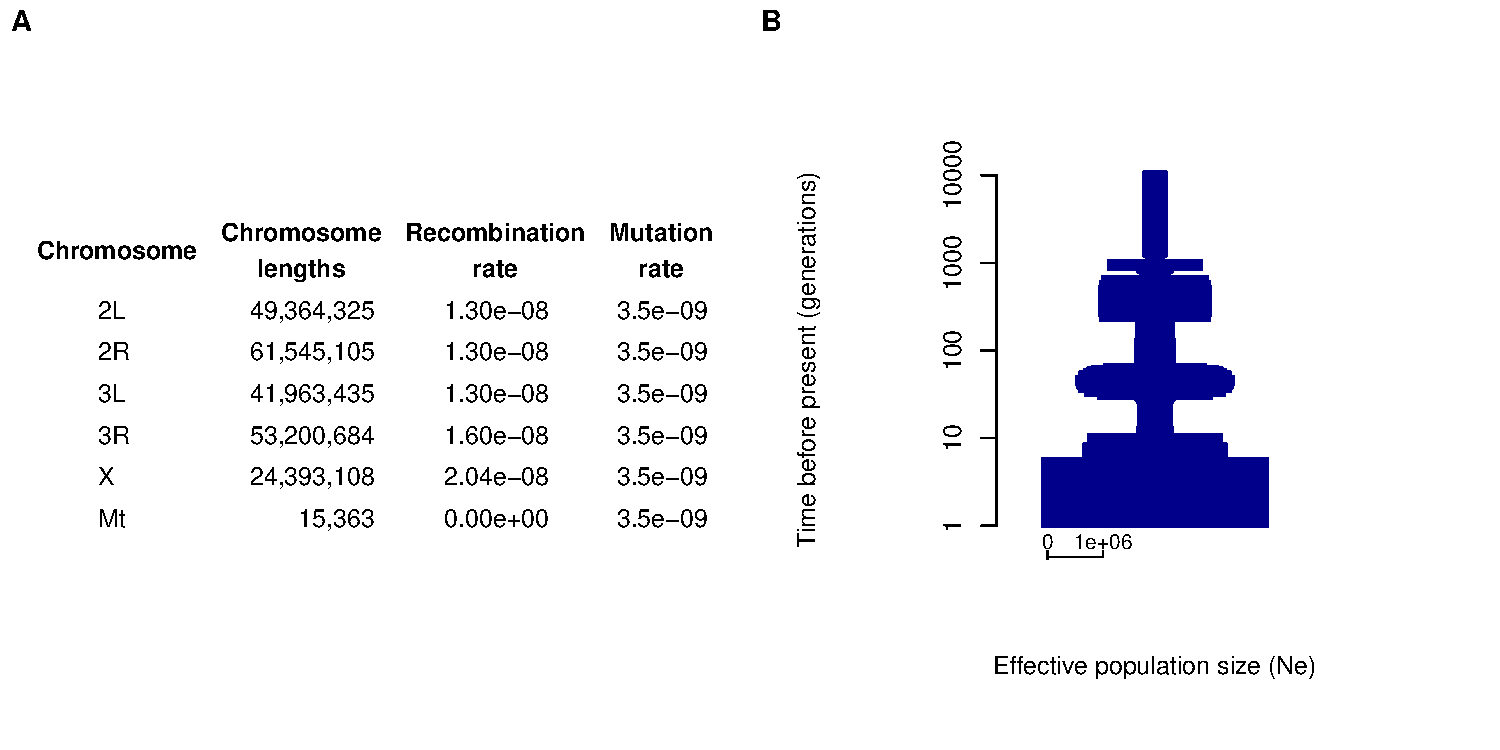
\includegraphics[width=\linewidth]{figs/anogam_demog_table}
	\caption{The species parameters and demographic model used for \emph{Anopheles gambiae} in the \stdpopsim catalog.
	(A) The parameters associated with the genome build and species, including
	chromosome lengths, average recombination rates (per base per generation),
	and average mutation rates (per base per generation).
	(B) A graphical depiction of the demographic model,
	which consists of a single population whose size changes throughout the past 11,260 generations in 67 time intervals. The width at each point depicts the effective population size (Ne), with the horizontal bar at the bottom indicating the scale for Ne=$10^6$.
		\label{fig:anogam} }
\end{figure}


\emph{Anopheles gambiae}, the African malaria mosquito, is 
a non-model organism whose population history has direct implications for human health.
Several large-scale studies in recent years have provided information about the
population history of this species on which population genomic simulations can be based \citep[e.g.,][]{Miles2017, clarkson2020genome}.
The genome assembly structure used in the species model is based 
on the AgamP4 \textbf{genome assembly} \citep{Sharakhova2007}, which 
was downloaded from Ensembl \citep{ensembl2021} via \stdpopsim's
utilities that interact with Ensembl. These utilities
make it easy to accurately retrieve basic genome information and construct the appropriate Python data structures.

% Ilan: I saw in the qc pr that there was some discussion about recombination rates
% for the x chrom. Anything worth reporting? Maybe the pending estimates from 
% the paper from Omar's group?

Estimates of average \textbf{recombination rates} for each of the chromosomes (excluding the mitochondrial genome)
were taken from a recombination map inferred by \citet{Pombi2006} which itself included information from
\citet{zheng1996integrated} (Figure \ref{fig:anogam}A).
As direct estimates of \textbf{mutation rate} (e.g., via mutation accumulation) do not currently exist for \emph{Anopheles gambiae},
we used the genome-wide average mutation rate of $\mu=3.5 \times 10^{-9}$ mutations per generation per site,
estimated by \cite{Keightley2009} for the closely related species, \textit{Drosophila melanogaster},
and used for analysis of \textit{A.~gambiae} data in \citet{Miles2017}.
To obtain an estimate for the default \textbf{effective population size} ($N_e$),
we used the formula $\theta=4\mu N_e$,
with the above mutation rate ($\mu=3.5 \times 10^{-9}$),
and a mean nucleotide diversity of $\theta\approx 0.015$,
as reported by \citet{Miles2017} for the Gabon population.
This resulted in an estimate of $N_e=1.07\times 10^{6}$,
which we rounded down to one million. 
These steps were documented in the code for the \stdpopsim species model,
to facilitate validation and future updates.
We acknowledge that some of these steps involve somewhat arbitrary choices,
such as the choice of the Gabon population and rounding down of the final value.
However, this should not be seen as a considerable source of misspecification,
since this value of $N_e$ is meant to provide only a rough approximation to
historic population sizes, which is to be overwritten by a more detailed demographic model.
\citet{Miles2017} inferred \textbf{demographic models} from \textit{Anopheles} samples from nine different populations (locations) using the stairway plot method \citep{Liu2015}.
We chose to include in \stdpopsim the model inferred from the Gabon sample, 
which consists of a single population whose size fluctuated from below 80,000
(an ancient bottleneck roughly 10,000 generations ago) to the present-day estimate of over 4 million individuals (Figure \ref{fig:anogam}B).
To convert the timescale from generations to years,
we used an average generation time of $1/11$ years,
as in \cite{Miles2017}.


All of these parameters were set in the appropriate source files in the \stdpopsim catalog,
accompanied by the relevant citation information,
and the model underwent the standard quality control process.
%Ilan: any issues worth mentioning that were raised in the QC?
The model may be refined in the future by adding more demographic models,
updating or refining the recombination map,
or updating the mutation rate estimates based on ones directly estimated for this species.
Note that even if the mutation rate is ever updated,
the demographic model mentioned above should still be associated with the current
mutation rate ($\mu=3.5 \times 10^{-9}$),
since this was the rate used in its inference.


\subsection*{\texorpdfstring{\emph{Bos taurus} (cattle)}{Bos taurus (cattle)}}
    \label{bos-taurus}

\emph{Bos taurus} (cattle) was added to the \stdpopsim catalog during the 2020 hackathon because of its agricultural importance. Agricultural species experience
strong selection due to domestication and selective breeding, leading
to a reduction in effective population size. These processes,
as well as admixture and introgression, produce patterns
of genetic variation that can be very different from typical model
species \citep{Larson2013}. These processes have occurred over a
relatively short period of time, since the advent of agriculture roughly 10,000 years ago, and they have increasingly intensified over the years to improve food production \citep{Gaut2018,MacLeod2013}. High quality genome assemblies are now
available for several breeds of cattle \citep[e.g.,][]{Rosen2020, Heaton2021,
Talenti2022} and the use of genomic data has become ubiquitous
in selective breeding \citep{Meuwissen2001,MacLeod2014, Obsteter2021, Cesarani2022}.
Modern cattle have extremely low and declining genetic diversity,
with estimates of effective population size around 90 in the early 1980s \citep{MacLeod2013, VanRaden2020, Makanjouloa2020}.
On the other hand, the ancestral effective population size is estimated to be roughly $N_e=62,000$ \citep{MacLeod2013}.
This change in effective population size presents a challenge for demographic inference, 
selection scans, genome-wide association, and genomic prediction
\citep{MacLeod2013,MacLeod2014,Hartfield2022}. 
For these reasons, it was useful to develop a detailed simulation model for cattle to be added to the \stdpopsim catalog.

We used the most recent \textbf{genome assembly}, ARS-UCD1.2
\citep{Rosen2020}, a constant \textbf{mutation rate} \(\mu=1.2\times 10^{-8}\) for all chromosomes \citep{Harland2017}, 
and a constant \textbf{recombination rate} \(r=9.26 \times 10^{-9}\) for all chromosomes other than the mitochondrial genome \citep{Ma2015}.
With respect to the \textbf{effective population size}, it is clear that simulating with either 
the ancestral or current effective population size will not generate realistic genome structure and diversity \citep{MacLeod2013,Rosen2020}.
Since \stdpopsim  does not allow for a missing value of $N_e$,
we chose to set the species default $N_e$ to the ancestral estimate of $6.2\times 10^4$.
However, we strongly caution that
simulating the cattle genome with any fixed value for $N_e$ will generate unrealistic patterns of genetic variation,
and recommend using a reasonably detailed demographic model.
We implemented the \textbf{demographic model} of the Holstein breed, which was
inferred by \cite{MacLeod2013} from runs of homozygosity in the whole-genome sequence of two iconic bulls.
This demographic model specifies the reduction from the ancestral effective population size ($N_e=62,000$) beginning around 33,000 generations ago, consisting of a series of 13 instantaneous population size changes, ultimately reaching the current effective population size ($N_e=90$) in the 1980s \citep[taken from Supplementary Table S1 in][]{MacLeod2013}.
To convert the timescale from generations to years, we used an average \textbf{generation time} of $5$ years \citep{MacLeod2013}.
Note that this demographic model does not capture the intense selective breeding since the 1980s that has even further reduced the effective population size of cattle \citep{MacLeod2013, VanRaden2020, Makanjouloa2020}. These effects can be modeled with
downstream breeding simulations \citep[e.g.,][]{Gaynor2020}.


When setting up the parameters of the demographic model, we noticed that the inference by \cite{MacLeod2013} assumed a genome-wide fixed recombination rate of \(r=10^{-8}\), and a fixed mutation rate \(\mu=9.4 \times 10^{-9}\) (considering also sequence errors).
The more recently updated mutation rate assumed in the species model \citep[\(1.2\times 10^{-8}\) from][]{Harland2017}
is thus \(28\%\) higher than the rate used for inference.
As a result, if one were to simulate the demographic model with the species' default mutation rate, they would produce synthetic genomes with considerably higher sequence diversity than actually observed in real genomic data.
To address this, we specified a mutation rate of \(\mu=9.4 \times 10^{-9}\) in the demographic model,
which then overrides the species' mutation rate when this demographic model is applied in simulation.
The issue of fitting the rates used in simulation with those assumed during inference was discussed during the independent review of this demographic model, and it raised an important question about recombination rates. Since \cite{MacLeod2013} use runs of homozygosity to infer the demographic model, their results depends on the assumed recombination rate. The recombination rate assumed in inference (\(r=10^{-8}\)) is \(8\%\) higher than the one used in the species model (\(r=9.26\times 10^{-9}\)). In its current version, \stdpopsim does not allow specification of a separate recombination rate for each demographic model, so we had no simple way to adjust for this. Future versions of \stdpopsim will enable such flexibility. Thus, we note that genomes simulated under the demographic model as currently implemented in \stdpopsim 
might have slightly higher linkage disequilibrium than observed in real cattle genomes.
However, we anticipate that this would affect patterns less
than selection due to domestication and selective breeding,
which are as of yet not modeled at all in \stdpopsim simulations.

\section*{Conclusion}
    \label{conclusion}

As our ability to sequence genomes continues to advance, the need for
population genomic simulation of new model and non-model organisms is becoming acute.
So too is the concomitant need for an expandable framework for implementing such simulations and guidance for how to do so.
Generating realistic whole-genome simulations presents significant challenges
in coding and the choice of parameter values on which to base the simulation.
\Stdpopsim is a resource that is uniquely poised to address these 
challenges as it provides easy access to state-of-the-art simulation engines and practices and an easy procedure for including new species genomes.
Moreover, the choices of new species to include are driven by the
needs of the population genomics community. In this manuscript we 
describe the expansion of \stdpopsim in two ways:
the addition of new features to the simulation framework that incorporate new evolutionary processes,
such as non-crossover recombination, which broaden the diversity of species that can
be realistically modeled; and the considerable expansion of the catalog itself
to include more species and demographic models. 

We also formulated a series of guidelines for implementing
population genomic simulations, which are based on
insights from the community-driven process of expanding the \stdpopsim catalog.
These guidelines specify the basic requirements for generating a useful chromosome-level simulation for a given species, as well as the rationale behind these requirements.
We also discuss special considerations for collecting relevant information from the literature,
and what to do if some of that information is not available.
Because this process is quite error-prone,
we encourage everyone implementing simulations to have their
parameter choices and implementation reviewed by at least one other
researcher.
These steps can be followed if you are implementing a simulation independently for your own use,
or, as we encourage, when you add your simulation code to \stdpopsim,
to ensure its robustness and make it available for future standardized research.
Currently, large-scale efforts such as the Earth Biogenome
and its affiliated project networks are generating tens of thousands of genome
assemblies. Each of these assemblies
will become a candidate for inclusion into the
\stdpopsim catalog following the steps we have outlined above,
assuming it satisfies our baseline requirements.
As annotations of those genome assemblies improve over time this information too can easily be added to the \stdpopsim catalog.

One of the important objectives of the PopSim consortium is to leverage \stdpopsim as means to promote education and inclusion of new communities into
computational biology and software development.
We are keen to use outreach, such as the workshops and hackathons described here, 
as a way to grow the \stdpopsim catalog and library and
democratize the development of population genomic simulations in general.
We predict that the increased use of whole-genome simulations in non-model species will lead to an improvement in inference methods,
which traditionally have been quite narrowly focused on well-studied model organisms.
Thus, we hope that further expansion of \stdpopsim will improve the ease and reproducibility of research across a larger number of systems,
while simultaneously expanding the community of software developers among population and evolutionary geneticists.


\section*{Acknowledgements}\label{acknowledgements}

%Ilan: anyone else to acknoweldge?
We wish to thank the dozens of workshop attendees,
and especially to the two dozen or so hackathon members,
whose combined feedback motivated many of the updates made to \stdpopsim in the past two years.

\section*{Funding}
    \label{funding}

%Ilan: I reordered this baed on author order, but we can reconsider, if needed
M.~Elise Lauterbur was supported by an NSF Postdoctoral Research Fellowship \#2010884.
Gregor Gorjanc was supported by the University of Edinburgh and BBSRC grant to The Roslin Institute (BBS/E/D/30002275).
Franz Baumdicker was supported by the Deutsche Forschungsgemeinschaft (DFG, German Research Foundation) under Germany’s Excellence Strategy – EXC 2064/1 – Project number 390727645, and EXC 2124 – Project number 390838134.
Ryan N. Gutenkunst was supported by NIH award R01GM127348.
Andrew D. Kern and Peter L. Ralph were supported by NIH award R01HG010774.

\bibliography{references}
\end{document}
